% Pré-visualizar código-fonte

%% LyX 2.1.4 created this file.  For more info, see http://www.lyx.org/.
%% Do not edit unless you really know what you are doing.
\documentclass[12pt,brazil]{article}
\usepackage{amsmath}
\usepackage{mathptmx}
\usepackage{helvet}
\usepackage{courier}
\usepackage{newtxmath}
\renewcommand{\familydefault}{\rmdefault}
\usepackage[T1]{fontenc}
\usepackage[utf8]{inputenc}
\usepackage[a4paper]{geometry}
\geometry{verbose,tmargin=3cm,bmargin=2cm,lmargin=3cm,rmargin=2cm,footskip=1cm}
\pagestyle{plain}
\setlength{\parskip}{\bigskipamount}
\setlength{\parindent}{0pt}
\usepackage{array}
\usepackage{pifont}
\usepackage{float}
\usepackage{booktabs}
\usepackage{textcomp}
\usepackage{graphicx}
\usepackage{setspace}
\usepackage{nomencl}
% the following is useful when we have the old nomencl.sty package
\providecommand{\printnomenclature}{\printglossary}
\providecommand{\makenomenclature}{\makeglossary}
\makenomenclature
\setstretch{1.5}

\makeatletter

%%%%%%%%%%%%%%%%%%%%%%%%%%%%%% LyX specific LaTeX commands.
%% Because html converters don't know tabularnewline
\providecommand{\tabularnewline}{\\}

%%%%%%%%%%%%%%%%%%%%%%%%%%%%%% Textclass specific LaTeX commands.
\numberwithin{figure}{section}
\numberwithin{table}{section}

%%%%%%%%%%%%%%%%%%%%%%%%%%%%%% User specified LaTeX commands.
%\usepackage{hyperref}
%

%%%%%%%%%%%%%%% MATRIX LABEL %%%%%%%%%%%%%%%%%%

\usepackage{titlesec}
\usepackage{amsmath}
\usepackage{lipsum}
\usepackage{indentfirst}
\usepackage{mathtools}
\usepackage{nomencl}
\usepackage{setspace}
\usepackage{empheq}
\usepackage{longtable}
\usepackage{steinmetz,environ}
\usepackage{colortbl}
\usepackage{graphicx}
\usepackage{caption}
\usepackage[table,usenames,dvipsnames]{xcolor}

\definecolor{celeste1}{RGB}{0,154,205}
\definecolor{verde5}{RGB}{0,150,0}
\definecolor{verde1}{RGB}{0,200,0}
\definecolor{firebrick}{RGB}{178,34,34}
\definecolor{crimson}{RGB}{220,20,60}
\definecolor{reda}{RGB}{220,20,70}
\definecolor{sea}{RGB}{46,139,87}
\definecolor{rosadito}{RGB}{255,192,203}
\definecolor{naranjita}{RGB}{255,159,0}
\definecolor{royalblue}{RGB}{0,35,102}
\definecolor{azvi}{RGB}{148,0,211}

%%%%%%%%%%%%% CORES
\definecolor{titulo}{RGB}{60,76,148}
\definecolor{section}{RGB}{148,0,211}
\definecolor{refFig}{RGB}{120,120,120}

%%%%%%%%%%%%%
%HYFFF
\PassOptionsToPackage{hyphens}{url}


\usepackage{multicol}
\usepackage{array}
\usepackage{multirow} 
\setlength{\columnsep}{0.5cm}
\usepackage[titletoc]{appendix}
\usepackage{url}


\usepackage{pgf}
\usepackage{tikz}
\usetikzlibrary{arrows,shapes,automata,petri}

% tabela longa que quebra entre p\'aginas
\usepackage{longtable}
%identando
%\usepackage{indentfirst}
%imagen en negritas
%\usepackage[labelfont={it,rm}, tableposition=top]{caption}
%\usepackage[labelfont={it,rm}]{caption}
%%%%%%%%%%%%%%%%
%%%PACKEGE CAPTION
%%%%%%%%%%%%%%%%



\DeclareCaptionFont{colorFigure}{\color{refFig}{}}
\DeclareCaptionFont{colorTable}{\color{refFig}{}}
\captionsetup[figure]{labelfont={bf,footnotesize,colorFigure},textfont={it,footnotesize},format=hang}%%
%labelsep=period}
\captionsetup[table]{labelfont={bf,footnotesize,colorTable}, format=hang,textfont={it,footnotesize}}
%%%%%%%%%%%%%%%%%%%%%%%%%%%%%%%%
%%%%Package SECTSTY
%Para centrar el capitulo
\usepackage{sectsty}
%\chapterfont{\centering}
%cambiar tamanho das fontes
\sectionfont{\fontsize{14}{14}\selectfont\color{black}}
\subsectionfont{\fontsize{13}{13}\selectfont\color{black}}
\subsubsectionfont{\fontsize{12}{12}\selectfont\color{black}\em}
\usepackage[hang,flushmargin]{footmisc}
\usepackage{multicol}
\usepackage{tikz}
\usepackage[siunitx]{circuitikz}
\usepackage[thinlines]{easytable}
\setlength{\extrarowheight}{2pt}
\renewcommand*\arraystretch{1}

%\renewcommand{\theequation}{\thesection.\arabic{equation}}
\usepackage{varioref}
\usepackage[hidelinks]{hyperref}
\usepackage{cleveref}

%\makeatletter
%\renewcommand\thefigure{\mbox{\thechapter-\arabic{figure}}}
%\makeatother
%\crefformat{figure}{#2\color{Cyan!40!blue}{{[Fig.~#1#3]}}}
%\crefformat{equation}{#2\color{Cyan!40!blue}{{[Eq.~#1#3]}}}
%\crefformat{table}{#2\color{Cyan!40!blue}{{[Tab.~#1#3]}}}


\crefname{section}{section}{sections}
\crefname{subsection}{subsection}{subsections}
\crefname{appendix}{appendix}{appendixes}
\crefformat{figure}{\textcolor{refFig}{#2(FIGURA~#1#3)}}
\crefformat{equation}{\textcolor{refFig}{#2(EQUAÇÃO~#1#3)}}
\crefformat{table}{\textcolor{refFig}{#2(TABELA~#1#3)}}
\crefformat{appendix}{\textcolor{refFig}{(#2ap.~#1#3)}}
\crefformat{section}{\textcolor{refFig}{#2(SEÇÃO~#1#3)}}
\crefformat{subsection}{\textcolor{refFig}{#2(SUBSEÇÃO~#1#3)}}

\usepackage{pstricks}

%textCIRCLED
\newcommand*\circled[1]{\tikz[baseline=(char.base)]{\node[shape=circle,draw,inner sep=2pt] (char) {#1};}}


%SPACING
%\titlespacing\section{0pt}{12pt plus 4pt minus 2pt}{0pt plus 2pt minus 2pt}
%\titlespacing\subsection{0pt}{12pt plus 4pt minus 2pt}{0pt plus 2pt minus 2pt}
%\titlespacing\subsubsection{0pt}{12pt plus 4pt minus 2pt}{0pt plus 2pt minus 2pt}


%======================================= FANCY HEADERS ===============================
\usepackage{fancyhdr}
\pagestyle{fancy}


\fancypagestyle{solo}{
	\fancyhf{}
	\fancyhead[RO]{}
	\fancyhead[LO]{}
	\cfoot{}
	\renewcommand{\headrulewidth}{0pt}
}

\fancypagestyle{demas}{
	\fancyhf{}
	\lhead{}
	\chead{}
	\rhead{\color{black}{\textbf{\footnotesize \thepage}}}
	\renewcommand{\headrulewidth}{0pt}
	\cfoot{}
}


\usepackage[pages=some]{background}
\backgroundsetup{
	scale=1,
	color=black,
	opacity=0.4,
	angle=0,
	contents={%
		\includegraphics[width=\paperwidth,height=\paperheight]{capa.png}
	}%
}


%=================== TIKS set ===================

\tikzset{
	place/.style={
		circle,
		thick,
		draw=blue!75,
		fill=blue!20,
		minimum size=6mm
	},
	transition/.style={
		rectangle,
		thick,
		fill=black,
		minimum width=8mm,
		inner ysep=2pt
	}
}
%\usepackage{kbordermatrix, blkarray}
%\renewcommand{\kbldelim}{[}
%\renewcommand{\kbrdelim}{]}


%\usepackage{pgf}
%\usepackage{tikz}


%%%%%%%%%%%%%%%%%%%%%%%%%%%PARRAFO

\setlength{\parindent}{1.9cm}
\setlength{\parskip}{1.5pt}
%\renewcommand{\baselinestretch}{1.5}



%% NOMENCLATURA
\usepackage{nomencl}
\usepackage{etoolbox}
\usepackage{enumitem}
\makenomenclature
\makeatletter
\patchcmd{\thenomenclature}{\section*}{\section*}{}{}
\makeatother

\usepackage[alf, abnt-verbatim-entry=no]{abntex2cite}
\urlstyle{tt}

\AtBeginDocument{
	\def\labelitemi{\scriptsize\ding{110}}
	\def\labelitemii{\ding{68}}
	\def\labelitemiii{\ding{103}}
}

\makeatother

\usepackage{babel}
\begin{document}
	
	
	\newcommand*\ntcc{Extração, Classificação e Reconhecimento de Padrões
		de Informação Contida em Artigos Acadêmicos Utilizando Mineração Web
		de Conteúdo e Mineração Web de Uso}
	
	\newcommand*\nautor{Ken Esparta Ccorahua}
	
	\newcommand{\token}{
		{
			\em{token}
		}
	}
	
	\newcommand{\fonteProp}{
		{
			\scriptsize{\em{Fonte: Autoria própria.\\\vspace{0.2em}}}
		}
	}
	
	\newcommand{\fonte}[1]{
		{
			\scriptsize{\em{Fonte:~Adaptado~de~#1.\\\vspace{0.2em}}}
		}
	}
	
	\newcommand{\imgFonte}[2]{
		{
			\scriptsize{\em{Fonte:~#1\\\vspace{0.2em}}}
		}
	}
	
	\newcommand{\imgFontSVG}[2]{
		\centering
		{
			\scriptsize{\em{Fonte:~#1\vspace{-0.8em}}}
		}
		\input{#2}
		\vspace{-1em}
	}
	
	\newcommand{\arq}[1]{\fcolorbox{gray!80}{gray!15}{\texttt{#1}}}
	%\renewcommand{\lstlistingname}{Listagem}
	
	\newcommand*\tcc{
		\textbf{
			\textcolor{black}{
				{\Large{}
					\ntcc
				}}
			}
		}
		
		
		
		\begin{titlepage}
			
			\noindent \begin{center}
				
\includegraphics[scale=0.1]{img/LOGO_PNG}
				\par\end{center}
			
			\vspace{-1.1cm}
			\begin{center}\textrm{\color{black}{
						\vspace{-0.08cm}
						{\textsc {\normalsize{}Universidade Federal Do Ceará}}\\
						\vspace{-0.3cm}
						{\em {Campus de Sobral}}}}
			\end{center}
			
			\begin{center}
				\vspace{1cm}
				{\large{}Curso de Engenharia da Computação}
				\par\end{center}{\large \par}
			
			\vspace{2.5cm}
			
			
			\begin{center}
				\large{\nautor}
				\par\end{center}
			
			\noindent \begin{center}
				\bigskip{}
				
				\par\end{center}
			
			\begin{center}
				{\textsc \tcc}
			\end{center}
			
			\noindent \begin{center}
				\vfill{}
				Sobral $-$ CE\\2016
				\par\end{center}
			
		\end{titlepage}
		
		\clearpage{}
		
		\newpage{}
		
		\thispagestyle{empty}
		
		
		
		\begin{center}
			%%%%%%
			\nautor
			%%%%%
			
		\end{center}
		
		\noindent \begin{flushleft}
			\vfill{}
			
			\par\end{flushleft}
		
		\begin{center}
			%%%%%%
			{\textsc { \textbf {\large{} \ntcc } }}
			%%%%%
			
		\end{center}
		
		\noindent \begin{flushleft}
			\vfill{}
			
			\par\end{flushleft}
		
		\begin{flushright}
			\begin{minipage}[t]{0.48\columnwidth}%
				Memorial de Monografia apresentado à disciplina de Seminário de Monografia
				do Curso Engenharia da Computação como requisito parcial para obtenção
				do grau Engenheiro da Computação na Universidade Federal do Ceará,
				\emph{campus} Sobral.%
			\end{minipage}
			\par\end{flushright}
		
		\noindent \begin{flushleft}
			\vfill{}
			\begin{tabular}{l}
				\textbf{Orientador}\tabularnewline
				\hline 
				Prof. Dr. Fernando Rodrigues de Almeida Júnior\tabularnewline
				\tabularnewline
				\textbf{Coorientador}\tabularnewline
				\hline 
				Prof. Dr. Márcio André Baima Amora\tabularnewline
			\end{tabular}\vfill{}
			
			\par\end{flushleft}
		
		\noindent \begin{center}
			Sobral $-$ CE, julho de 2016
			\par\end{center}
		
		\clearpage{}
		
		\newpage{}
		
		\cleardoublepage
		\phantomsection
		\setcounter{page}{1}
		\thispagestyle{empty}
		\phantomsection
		\addcontentsline{toc}{section}{Lista de Figuras}
		
		\listoffigures
		
		
		\clearpage{}
		
		\newpage{}
		
		\cleardoublepage
		\phantomsection
		\setcounter{page}{1}
		\thispagestyle{empty}
		\phantomsection
		\addcontentsline{toc}{section}{Lista de Tabelas}
		
		\listoftables
		
		
		\newpage{}
		
		\clearpage{}
		
		\cleardoublepage
		\phantomsection
		\thispagestyle{empty}
		\phantomsection
		\addcontentsline{toc}{section}{Lista de abreviaturas e siglas}
		\renewcommand{\nomname}{Lista de abreviaturas e siglas} 
		
		\printnomenclature[2.5cm]{}
		
		\newpage{}
		
		\clearpage{}
		
		\cleardoublepage
		\phantomsection
		\thispagestyle{empty}
		\phantomsection
		
		\tableofcontents{}
		
		\clearpage{}
		
		\pagestyle{demas}
		
		
		\section{Introdução}
		
		A World Wide Web (WWW) \nomenclature[WWW]{WWW}{World Wide Web} ou
		comumente denominada Web, vem crescendo nos últimos vinte anos. Aplicações
		Web tornam-se populares e um dos motivos é que o navegador permite
		executá-las a partir de qualquer tipo de dispositivo, em outras palavras,
		o sistema operacional não influencia a aplicação no tempo de execução.
		
		Tanto dados estruturados como dados não estruturados trafegam pela
		Web. O próprio documento HTML\nomenclature[HTML]{HTML}{HyperText Markup Language}
		renderizado no navegador é uma fonte de dados tais como endereços
		Web, informações pessoais, meta-tags, folhas de estilos, arquivos
		XML\nomenclature[XML]{XML}{Extensible Markup Language}, arquivos
		JSON\nomenclature[JSON]{JSON}{JavaScript Object Notation}, entre
		outros. Não obstante, os dados que estão contidos em um documento
		HTML possuem informações relevantes que podem ser mineradas. É nesse
		contexto onde se aplica o processo de mineração de dados.
		
		Existem também os Web logs, que são as informações armazenadas através
		do tempo relacionadas ao servidor que estão em ordem cronologicamente
		descendente. Para minerar os dados no Web log, utiliza-se a mineração
		Web de uso. No presente trabalho utiliza-se o Web log de artigos da
		Wikipédia.
		
		A teoria apresentada no trabalho realiza-se através de uma rede de
		Petri, onde os estados são as áreas da Ciência da Computação a serem
		atingidas e as transições são as técnicas e o embasamento teórico
		requeridos para passar ao estado seguinte. Começa-se pela Soft Computing
		(SC\nomenclature[SC]{SC}{Soft Computing}), que é uma área das Ciências
		da Computação que permite resolver problemas com uma abordagem orientada
		à tolerância de imprecisões. Em seguida, aborda-se a teoria relacionada
		com o aprendizado de máquina, que, juntamente com as técnicas de descobrimento
		de conhecimento, dão origem às técnicas de mineração de dados. Finalmente,
		apresenta-se a mineração Web de conteúdo (ou Web Content Mining\nomenclature[WCM]{WCM}{Web Content Mining})
		e mineração Web de uso (ou Web Usage Mining\nomenclature[WUM]{WUM}{Web Usage Mining}),
		cujas técnicas são utilizadas no trabalho.
		
		Existe o problema da desconfiança do conteúdo nos artigos da Wikipédia
		e também de outros na internet. A proposta neste trabalho é o desenvolvimento
		de uma aplicação Web de busca na internet que tem como objetivo principal
		a mineração de informação em artigos acadêmicos se baseando em Web
		logs da Wikipédia e, finalmente, mostrando como resultado ao usuário
		endereços Web de artigos de confiança.
		
		A mineração será dada em dois níveis. No primeiro nível tem-se a mineração
		de uso nos Web logs de artigos da Wikipédia e no segundo nível, a
		mineração de conteúdo de outros sites onde também são oferecidos artigos
		acadêmicos. O resultado da pesquisa que o usuário faz na aplicação
		Web final é a junção da mineração de uso de Web logs da Wikipédia
		e a mineração de conteúdo de artigos acadêmicos externos a ela.
		
		
		\section{Objetivo}
		
		
		\subsection{Objetivo geral}
		
		Extrair, classificar e reconhecer padrões nas informações contidas
		em artigos acadêmicos, a partir de uma busca efetuada pelo usuário
		do sistema proposto no trabalho, tendo como base os Web logs da Wikipédia
		e utilizando técnicas de mineração Web de conteúdo e mineração Web
		de uso.
		
		
		\subsection{Objetivos específicos}
		
		\begin{itemize}[leftmargin=1.9cm,labelwidth=2cm,labelindent=1.5em,labelsep=0.55cm]
			
			\item Mostrar ao usuário final que os resultados da busca efetuada
			são artigos de confiança do ponto de vista acadêmico.
			
			\item Utilizar técnicas de classificação de conteúdo de artigos Web
			da Wikipédia no aprimoramento da utilização de algoritmos de aprendizado
			de máquina.
			
			\item Utilizar técnicas de aprendizado de máquina para reconhecer
			padrões a partir de logs gerados pelos servidores da Wikipédia.
			
			\item Aplicar a fundamentação teórica relacionada com redes neurais
			para ajudar a geração de conhecimento dos dados extraídos de artigos
			acadêmicos.
			
			\item Implementar o processo de Mineração de dados CRISP-DM, proposto
			em \cite{pete_2000}, para gerar um modelo sólido que garanta o funcionamento
			da mineração de conteúdo e de uso nas páginas da Wikipédia.
			
			\item Mostrar que a Web é uma poderosa ferramenta para adquirir conhecimento
			relevante relacionado com artigos acadêmicos de sites semelhantes
			à Wikipédia. 
			
		\end{itemize}
		
		
		\section{Justificativa}
		
		As aplicações Web estão sendo amplamente utilizadas pelas empresas
		principalmente porque são multiplataforma e podem ser acessadas a
		partir de qualquer lugar do mundo desde que exista uma conexão com
		a internet. Computação na nuvem como: Amazon Web Service, Heroku,
		Digital Ocean, entre outras, estão crescendo no mercado. O próprio
		trabalho utiliza os serviços da Digital Ocean para alocar os códigos
		de teste e do produto final.
		
		Assim como as aplicações Web estão crescendo, o mercado relacionado
		com comércio eletrônico também. É imprescindível que uma empresa que
		vende produtos e serviços através de uma aplicação Web tenha dados
		das atividades que seus clientes realizam quando usam o aplicativo
		e isso pode ser feito utilizando a mineração Web de uso. Por outro
		lado, é necessário também que a empresa obtenha informação a partir
		de aplicações Web de outras empresas concorrentes para oferecer melhores
		ofertas aos clientes. Essa obtenção de informação é realizada utilizando
		técnicas de mineração Web de conteúdo.
		
		A lógica proposta no parágrafo anterior aplica-se também no trabalho,
		porém não possui abordagem comercial. O usuário final busca artigos
		utilizando o sistema Web, que é proposto no trabalho, o qual indexa
		outras páginas de artigos Web relacionadas com a busca utilizando
		mineração Web de conteúdo. O resultado é uma busca que retorna um
		conjunto de endereços Web com artigos de confiança considerando, além
		dos Web logs da Wikipédia, a informação de outros artigos acadêmicos.
		
		
		\section{Trabalhos relacionados}
		
		\begin{itemize}[leftmargin=1.9cm,labelwidth=2cm,labelindent=1.5em,labelsep=0.55cm]
			
			\item No artigo acadêmico intitulado \emph{“E-commerce Web page classification
				based on automatic content extraction”} referenciado em \cite{petprasit_2015},
			propõe-se o método Markov Random Field para reduzir o número de caraterísticas
			no conjunto de dados que foram extraídos da Web utilizando o método
			Subject Detection and Node Density. Em seguida, faz-se uma comparação
			de performance entre as redes neurais Radial Basis Function e Support
			Vector Machine com o método Naive Bayes.
			
			\item No artigo acadêmico intitulado \emph{“E-commerce website ranking
				using Semantic Web mining and neural computing”} referenciado em \cite{verma_2015},
			utilizam-se redes neurais, mineração Web de uso e de conteúdo para
			desenvolver uma aplicação Web de determinação de prioridade de diferentes
			páginas Web de comércio eletrônico.
			
			\item No artigo acadêmico intitulado \emph{“A framework for building
				Web mining applications in the world of blogs: A case study in product
				sentiment analysis”} referenciado em \cite{costa_2012}, descreve-se
			um framework desenvolvido na linguagem Java™ que utiliza os serviços
			da mineração Web semântica para ajudar a usuários de blogs na busca
			efetiva de informação relevante no mundo dos blogs. Esse framework
			utiliza uma interface de aplicação, um controlador de mineração de
			dados na Web (Web crawler) e um extractor de textos.
			
			\item No artigo acadêmico intitulado \emph{“Web Classification Mining
				Based on Radial Basis Probabilistic Neural Network”} referenciado
			em \cite{gao_2009}, utiliza-se o método K-Nearest Neighbor (KNN)
			modificado para treinar a rede neural do tipo Radial Basis Probabilistic;
			os dados utilizados para classificação e treinamento foram extraídos
			de mil páginas Web utilizando a mineração Web de conteúdo.
			
			\item No artigo acadêmico intitulado \emph{“Structured Web information
				extraction using repetitive subject pattern”} referenciado em \cite{thamviset_2012}
			propõe-se uma técnica semi supervisionada que cria um padrão de extração
			de dados de páginas Web de comércio eletrônico. O sistema é composto
			por um extrator de dados e um wrapper que traduz os conteúdos da Web
			para tabelas do tipo relacionais.
			
		\end{itemize}
		
		
		\section{Fundamentação teórica}
		
		Apresentam-se breves definições sobre os assuntos teóricos relacionados
		com a monografia, utiliza-se uma abordagem \emph{top-down} como pode-se
		observar na \cref{fig:organ_teorica}, mostra-se uma rede de Petri
		que representa a montagem teórica do presente trabalho, na qual o
		estado inicial é o mais genérico e o estado final é o mais específico. 
		
		\captionsetup{width=0.7\textwidth}
		\begin{figure}[h]
			\noindent \centering{}\caption{Estruturação do conhecimento para conseguir as ferramentas teóricas
				e técnicas relacionadas com o presente trabalho.\label{fig:organ_teorica}}
			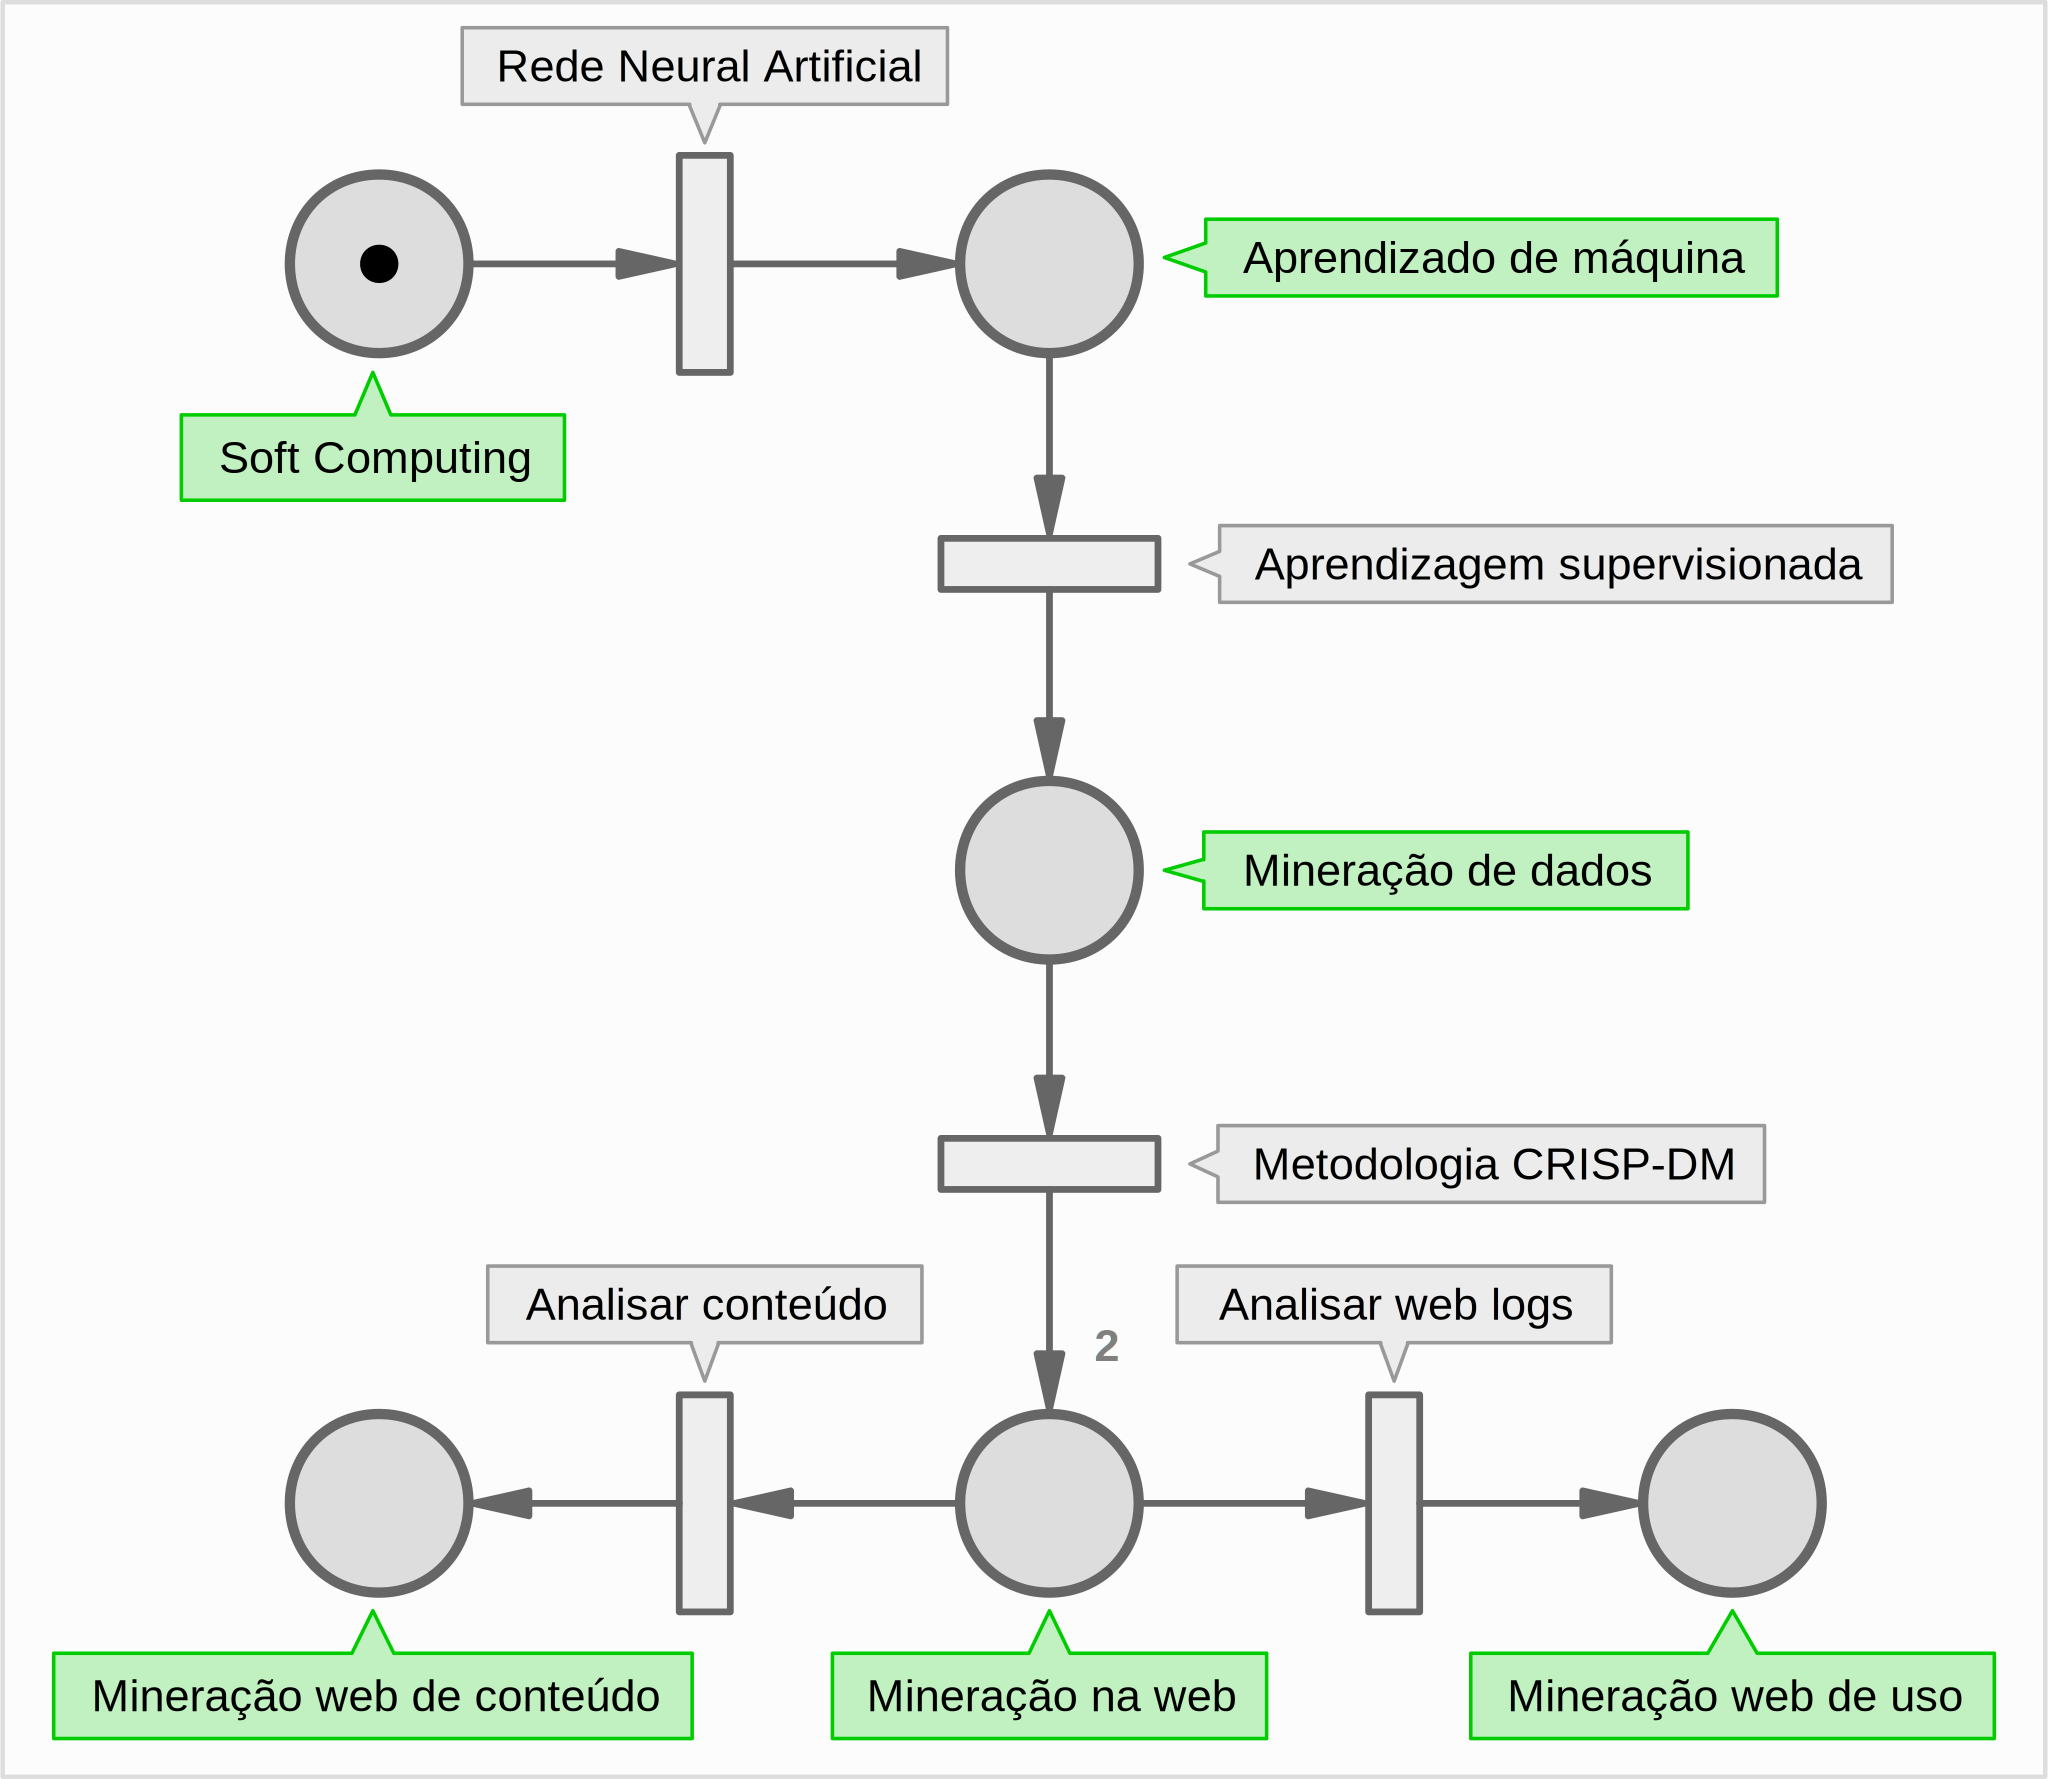
\includegraphics[scale=0.6]{img/rede_petri_teoria}\\\vspace{-0.1em}\fonteProp
		\end{figure}
		
		
		Na rede de Petri proposta, observa-se também que cada estado representa
		uma área das Ciências da Computação a qual possui ferramentas teóricas
		as quais serão adotadas para que a ficha posa ativar as transições.
		Cada transição representa uma ferramenta que será adquirida do estado
		anterior antes de passar ao próximo. Em outras palavras, a ficha pode
		passar somente ao estado seguinte quando uma ferramenta específica
		do estado anterior é definida para ser utilizada.
		
		
		\subsection{Soft computing}
		
		Existem dois tipos de paradigmas computacionais, a Soft Computing
		(SC) e a Hard Computing (HC\nomenclature[HC]{HC}{Hard Computing}),
		ambos os termos foram estabelecidos pela primeira vez pelo professor
		L. A. Zadeh no ano 1996. O HC trata sobre modelos precisos onde as
		soluções são atingidas imediatamente, por outra parte, a SC lida com
		modelos de aproximações e dá soluções a problemas complexos \cite{sivanandam_2004}.
		Como pode-se perceber, a HC é basicamente a computação convencional
		onde a solução dos problemas baseia-se nos princípios da precisão.
		Em contraste, o paradigma da SC trata sobre solucionar problemas utilizando
		modelos imprecisos que possuem certa porcentagem de aproximação.
		
		Cataloga-se a SC, em \cite{oded_2007}, como uma coleção de novas
		técnicas em inteligência artificial que exploram a tolerância para
		a imprecisão, incerteza, verdade parcial e manipulação de não linearidades
		para poder alcançar rastreabilidade, robustez e soluções de menor
		custo comparado com os métodos da HC, ou seja apresenta-se uma coleção
		de ferramentas aptas para minerar a Web porque esta encaixa-se nas
		definições de imprecisão, incerteza e veracidade duvidosa.
		
		\captionsetup{width=0.7\textwidth}
		\begin{figure}[h]
			\noindent \centering{}\caption{Principais componentes da família da SC.\label{fig:sc_comp}}
			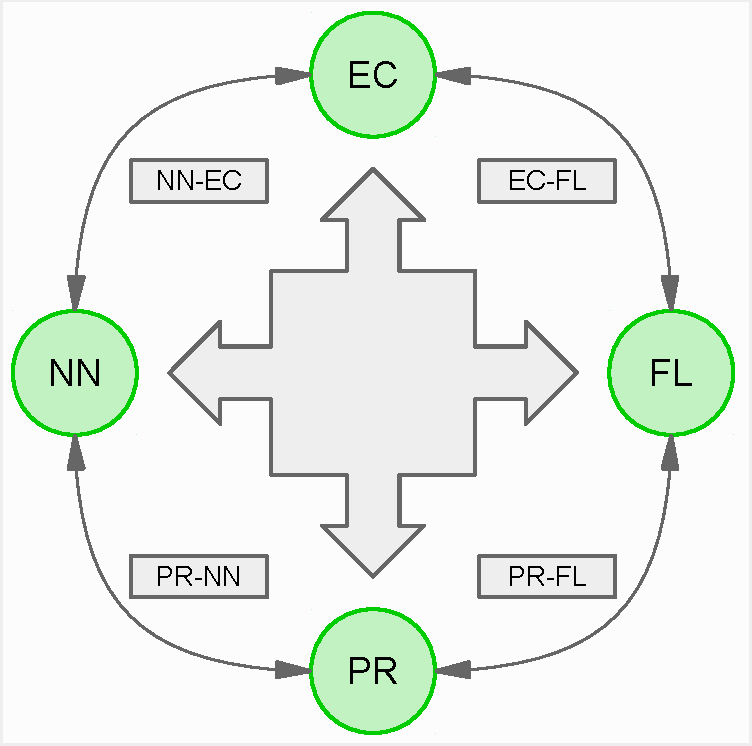
\includegraphics[scale=0.43]{img/soft_computing_family}\\\vspace{-0.1em}\fonte{\cite{kunjal_2013}}
		\end{figure}
		
		
		A SC está composta por técnicas como a rede neural (Neural Network\nomenclature[NN]{NN}{Neural Network}),
		computação evolucionária (Evolutionary Computing\nomenclature[EC]{EC}{Evolutionary Computing}),
		sistemas difusos (Fuzzy Systems\nomenclature[FS]{FS}{Fuzzy Systems})
		e raciocínio probabilístico (Probabilistic Reasoning\nomenclature[PR]{PR}{Probabilistic Reasoning}),
		como mostrado na \cref{fig:sc_comp}.
		
		As técnicas mostradas na \cref{fig:sc_comp}, nem sempre estão isoladas.
		Elas podem ser aplicadas ao mesmo tempo para resolver um mesmo problema,
		e isso denomina-se hibridação.
		
		Em \cite{zadeh_1996} define-se a SC como uma nova abordagem da computação
		a qual é análoga à habilidade marcante da mente humana para pensar
		e aprender sobre um entorno incerto e impreciso. A SC, segundo \cite{devendra_2008},
		é uma vertente da computação na qual pretende-se construir máquinas
		inteligentes e sábias. Pode-se observar na \cref{fig:top_down_abordagem}
		o desenvolvimento da SC, começando pela computação convencional, até
		chegar ao extremo de pensamento puro por parte de um computador, ou
		seja, o objetivo final da SC é projetar e desenvolver um computador
		que possa agir de forma semelhante aos seres humanos.
		
		\captionsetup{width=0.7\textwidth}
		\begin{figure}[H]
			\noindent \centering{}\caption{Desenvolvimento da SC.\label{fig:top_down_abordagem}}
			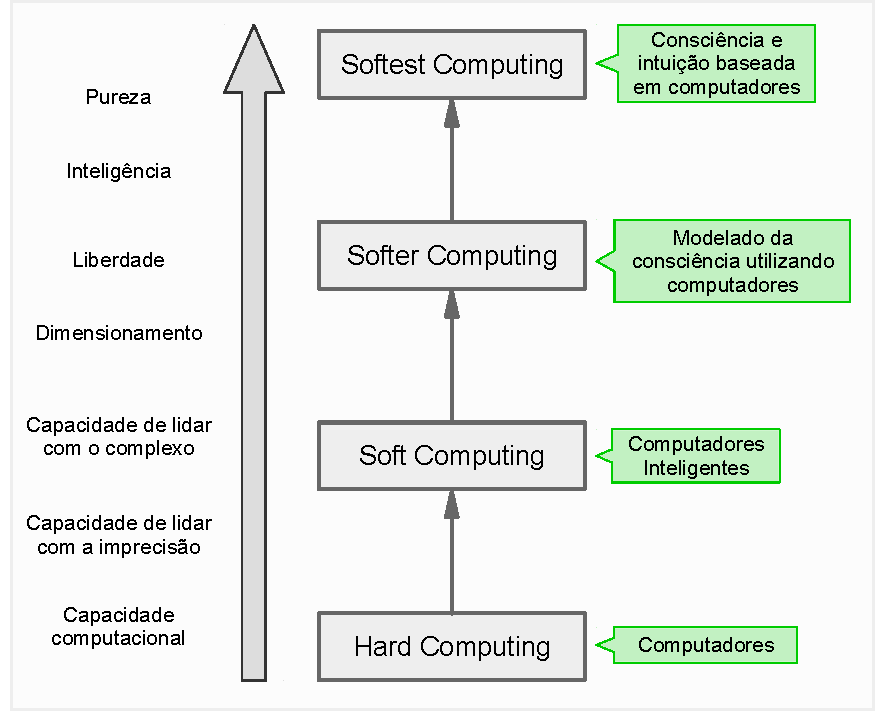
\includegraphics[scale=0.55]{img/abordagem_top_down}\\\vspace{-0.1em}\fonte{\cite{devendra_2008}}
		\end{figure}
		
		
		Para conseguir ativar a transição na rede de Petri da \cref{fig:organ_teorica}
		é necessário estabelecer a rede neural como técnica para poder passar
		ao estado seguinte que é o aprendizado de máquina.
		
		Uma rede neural artificial (ou simplesmente rede neural) é um modelo
		matemático simplificado de uma rede de neurônios biológicos. A unidade
		fundamental de uma rede neural é o neurônio que está interconectado
		com outros. Essas redes executam em paralelo uma tarefa global comum
		e possuem a habilidade de aprendizagem. Explica-se em \cite{kunjal_2013}
		que uma consequência da aprendizagem dos neurônios de uma rede neural
		é a aquisição de conhecimento de modo a torná-lo disponível para o
		uso. As caraterísticas básicas de uma rede neural são o paralelismo
		inerente, acesso à informação local, a semelhança entre suas componentes
		e o aprendizado incremental.
		
		
		\subsection{Aprendizado de máquina}
		
		\label{sec:aprendizado_maquina}
		
		A ficha encontra-se no seguinte estado, contendo já a teoria de uma
		rede neural. Nesta seção trata-se sobre as técnicas que serão adotadas
		do aprendizado de máquina (Machine Learning).
		
		O aprendizado automático ou aprendizado de máquina é um programa de
		computador que pode “aprender” de um conjunto de entradas disponíveis.
		Define-se, em \cite{kevin_2012}, que o aprendizado de máquina é um
		conjunto de métodos que podem detectar automaticamente padrões em
		um determinado conjunto de dados e, posteriormente, utilizar esse
		padrões descobertos para predizer dados futuros. Aprendizado é, grosseiramente
		falando, o processo de converter experiência em habilidade ou conhecimento
		\cite{shai_2014}. Aprender a partir de dados é o conceito fundamental
		do ML\nomenclature[ML]{ML}{Machine Learning}.
		
		O foco do ML é a modelagem do aprendizado e a adaptação (atividades
		de animais e humanos) num computador. Os métodos do ML são denominados
		“sub-simbólicos” porque não existem símbolos ou manipulação deles
		envolvidos, em contraste com a Inteligência Artificial, onde o computador
		manipula símbolos que refletem o entorno (processo simbólico) \cite{stephen_2015}.
		
		Tomando como ponto de partida que as máquinas aprendem a partir de
		dados, então, em \cite{stephen_2015} a ML trata sobre como fazer
		computadores modificarem ou adaptarem as suas ações de modo que estas
		se tornem mais precisas, onde a precisão é medida por quão bem a escolha
		de ações refletem as escolhas corretas.
		
		Em que momento precisa-se do ML?, responder esta pergunta é fundamental
		porque justifica a utilização dos conceitos de ML no trabalho. A resposta
		é dada em \cite{shai_2014}, onde sugere-se que os conceitos de ML
		devem ser utilizados em tarefas realizadas por humanos ou animais.
		De acordo com isso, precisa-se do ML para poder modelar os algoritmos
		deste trabalho; de modo que utilizam-se dados gerados pela interação
		humana com a Web a partir de buscas.
		
		De acordo com \cite{kevin_2012}, o aprendizado de máquina divide-se,
		usualmente, em aprendizado supervisionado, aprendizado não supervisionado
		e aprendizado por reforço. Na abordagem supervisionada ou preditiva
		do ML, tem-se como objetivo o aprendizado mapeando as saídas a partir
		das entradas, dado um conjunto de treinamento. A segunda abordagem
		de ML, a não supervisionada ou descritiva, tem como objetivo encontrar
		padrões e correlações entre os dados. Finalmente, a abordagem de aprendizado
		por reforço, trata-se do modo de agir ou se comportar diante uma situação
		de recompensa ou de punição.
		
		A atividade de classificar e extrair conhecimento a partir do conteúdo
		de páginas Web da Wikipédia justifica a escolha da utilização das
		ferramentas oferecidas pela abordagem supervisionada do aprendizado
		de máquina. Então, a ficha da rede de Petri passa para o seguinte
		estado sabendo que até esta subseção, juntando os conceitos revisados,
		está sendo utilizada uma rede neural com aprendizagem supervisionada.
		
		
		\subsection{Mineração de dados}
		
		\label{sec:mineracao_dados}
		
		A mineração de dados (data mining) é definida, segundo \cite{mohammed_2014},
		como o processo de descoberta intuitiva de novos padrões de interesse,
		assim como modelos preditivos, descritivos e compreensíveis.
		
		Em \cite{anand_2012} descreve-se a mineração de dados como a descoberta
		de modelos a partir de dados. Existem duas abordagens: a estatística
		e a do aprendizado de máquina. Para o presente trabalho utiliza-se
		a abordagem de aprendizado de máquina, esta decisão justifica-se na
		\cref{sec:aprendizado_maquina}. 
		
		Uma analogia da mineração de dados faz-se, em \cite{jiawei_2012},
		com a obtenção de ouro das rochas em uma mina. Ademais, enfatiza-se
		que o nome apropriado para mineração de dados é “conhecimento minerado
		a partir de dados”. Segundo \cite{jiawei_2012}, a descoberta de conhecimento
		a partir de dados (ou KDD do inglês knowledge discovery from data)
		é sinônimo de mineração de dados, não obstante em \cite{umair_2014}
		coloca-se o KDD, juntamente com o CRISP-DM e o SEMMA, como um tipo
		de processo relacionado com a mineração de dados, seguidamente, expõe-se
		uma breve descrição sobre eles:
		
		\begin{description}[style=multiline,leftmargin=2.5cm]
			
			\item [{KDD\nomenclature[KDD]{KDD}{knowledge discovery from data}}]
			É um modelo de processo que consiste na extração de conhecimentos
			escondidos a partir de um banco de dados. Deve ser um processo interativo
			e iterativo, possui cinco passos de desenvolvimento que se podem observar
			na \cref{fig:KDD}.
			
			\captionsetup{width=0.7\textwidth}
			\begin{figure}[H]
				\noindent \centering{}\caption{Uma visão geral dos passos que compõem o processo KDD.\label{fig:KDD}}
				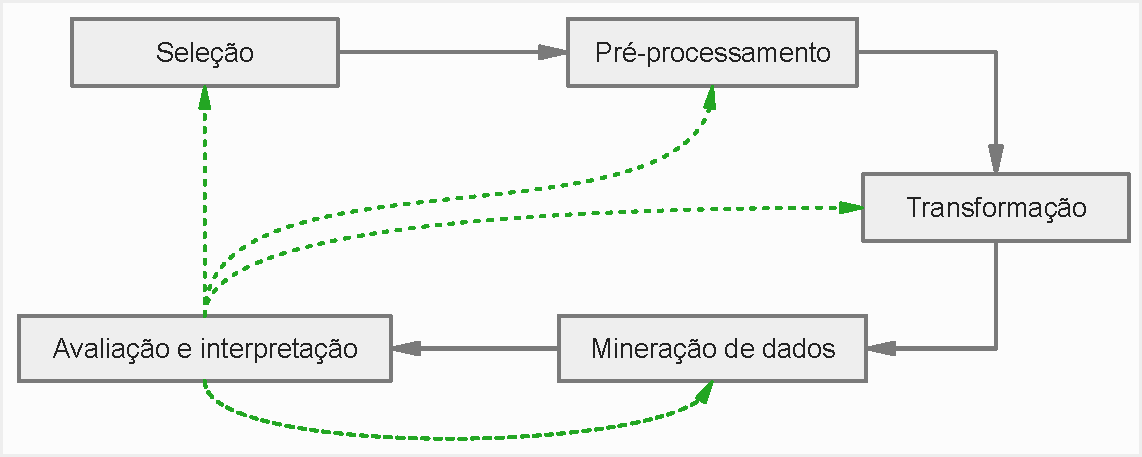
\includegraphics[scale=0.52]{img/kdd}\\\vspace{-0.1em}\fonte{\cite{fayyad_1996}}
			\end{figure}
			
			
			\item [{SEMMA\nomenclature[SEMMA]{SEMMA}{Sample, Explore, Modify, Model and Assess}}]
			Do acrônimo Sample, Explore, Modify, Model and Assess; que foi desenvolvido
			pelo instituto SAS\footnote{Statistical Analysis System, é o nome de uma empresa pioneira em Business
				intelligence. Disponível em \url{http://www.sas.com}}. Foca-se basicamente no desenvolvimento e manutenção de projetos
			de mineração de dados. Consiste em um ciclo altamente iterativo de
			cinco passos como pode-se verificar na \cref{fig:SEMMA}.
			
			\captionsetup{width=0.7\textwidth}
			\begin{figure}[H]
				\noindent \centering{}\caption{Metodologia SEMMA proposto pela SAS.\label{fig:SEMMA}}
				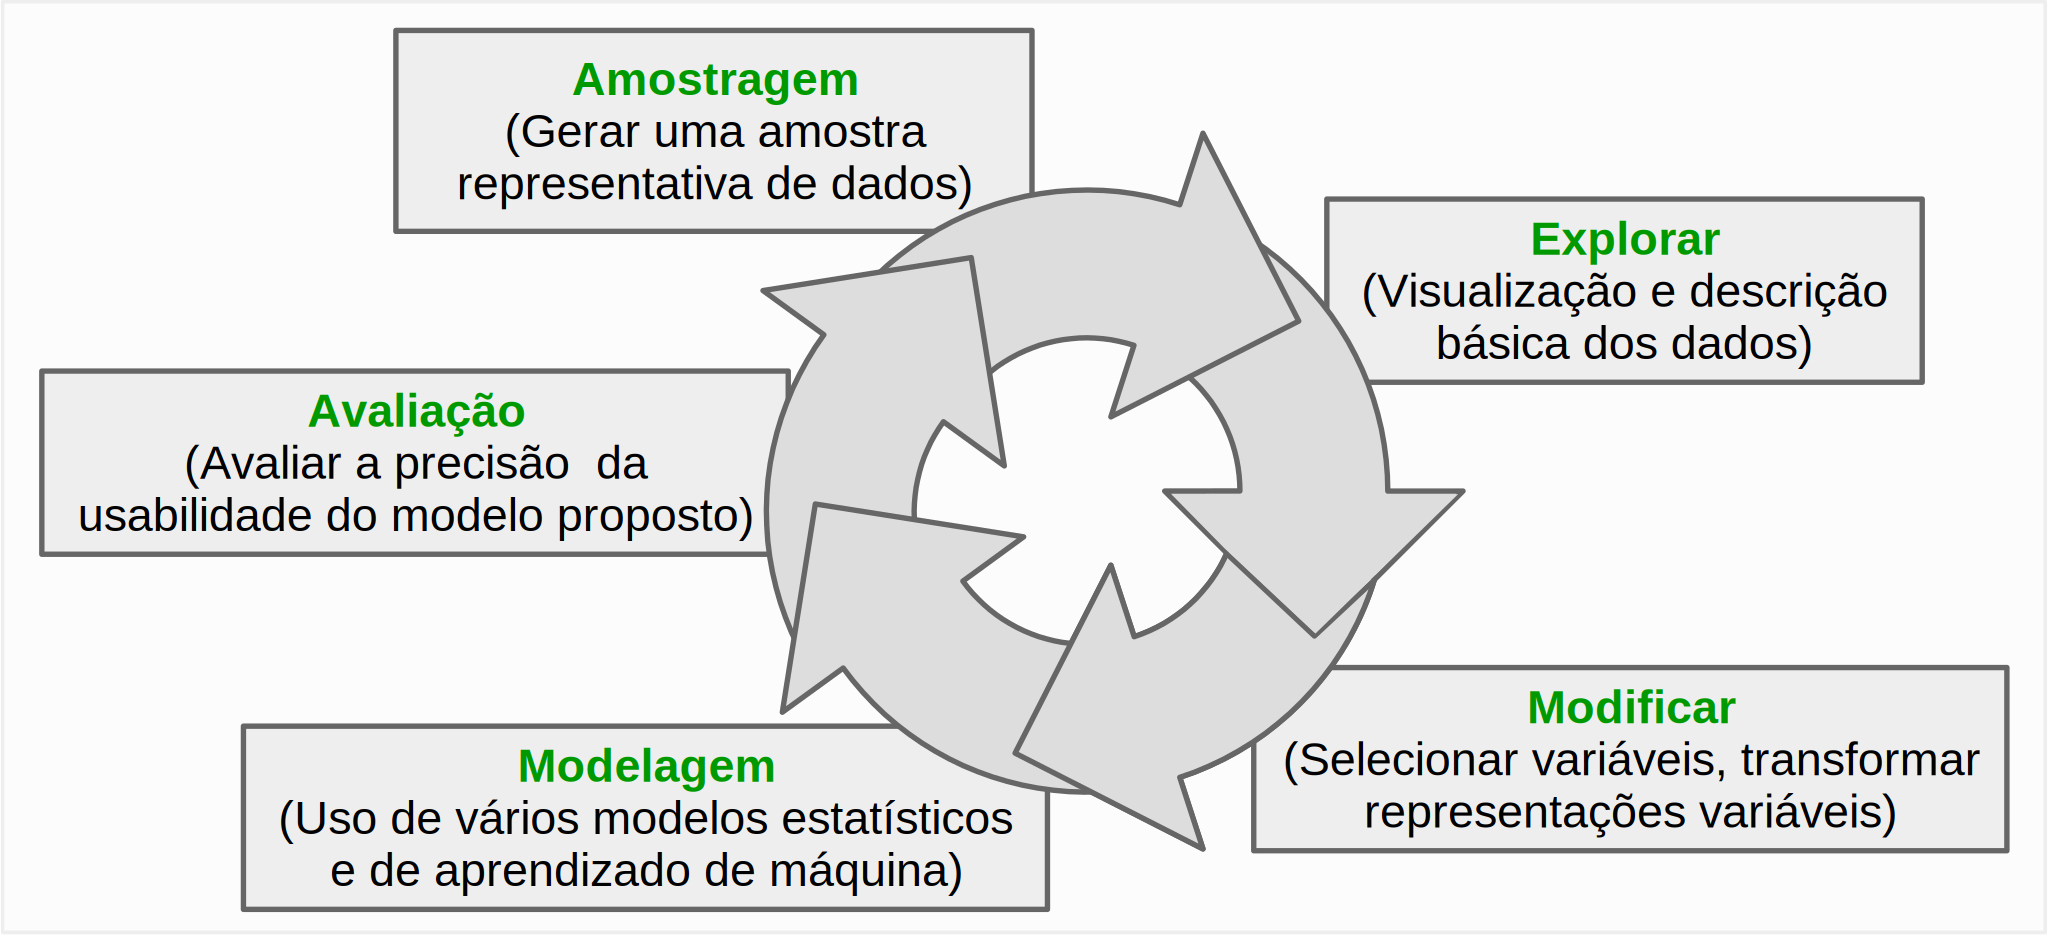
\includegraphics[scale=0.5]{img/semma}\\\vspace{-0.1em}\fonte{\cite{binus_2014}}
			\end{figure}
			
			
			\item [{CRISP-DM\nomenclature[CRISP-DM]{CRISP-DM}{Cross-Industry Standard Process for Data Mining}}]
			É um processo de mineração de dados que significa Cross-Industry Standard
			Process for Data Mining. Segundo \cite{pete_2000}, o processo foi
			concebido no ano 1996 pelas empresas DaimlerChrysler\footnote{É um fabricante de automóveis de passageiros e veículos comerciais.
				Disponível em \url{https://www.daimler.com}}, SPSS\footnote{É um software para análise estatística de dados, disponível em \url{http://www.ibm.com/analytics/us/en/technology/spss/}}
			e NCR\footnote{É uma empresa de tecnologia especializada em produtos para o varejo
				e setores financeiros, disponível em \url{http://www.ncr.com}}. É uma ferramenta que está constituída por seis processos cíclicos
			como se mostra na \cref{fig:CRISP-DM}. Segundo a pesquisa de \cite{gregory_2014}
			no site KDnuggets, pode-se observar na \cref{tab:crisp-dm_pesquisa}
			que o CRISP-DM é o método mais utilizado nos anos 2007 e 2014.
			
			\captionsetup{width=0.7\textwidth}
			\begin{figure}[H]
				\noindent \centering{}\caption{Metodologia CRISP-DM, utilizada no presente trabalho.\label{fig:CRISP-DM}}
				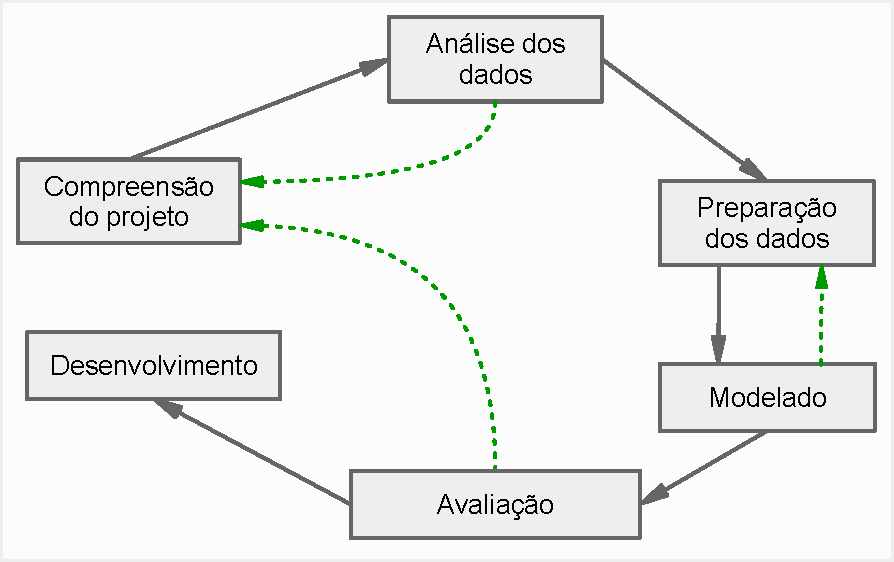
\includegraphics[scale=0.6]{img/crisp-dm}\\\vspace{-0.1em}\fonte{\cite{david_2008}}
			\end{figure}
			
			
		\end{description}
		
		Para passar ao seguinte estado da rede de Petri estabelecida, veja-se
		\cref{fig:organ_teorica}, é necessário adotar um tipo de processo
		de mineração de dados. Como é mencionado em \cite{david_2008}, nas
		três metodologias que foram abarcadas, não há obrigação de seguir
		de forma rígida seus respectivos passos. Afinal, optou-se por seguir
		a metodologia CRISP-DM. Na \cref{sec:materiais_metodos} vê-se a aplicação
		desta metodologia a partir do ponto de vista da proposta do trabalho.
		
		\captionsetup{width=0.8\textwidth}
		\begin{table}[H]
			\noindent \centering{}\caption{Pesquisa realizada com 200 pessoas sobre qual é a metodologia favorita
				utilizada nos projetos de mineração de dados, nos anos 2007 e 2014.
				\label{tab:crisp-dm_pesquisa}}
			\begin{tabular}{crr}
				\toprule 
				\textbf{Metodologia} & \textbf{Ano 2007 (\%)} & \textbf{Ano 2014 (\%)}\tabularnewline
				\midrule
				\midrule 
				CRISP-DM & 42.0 & 43.0\tabularnewline
				\midrule
				Própria & 19.0 & 27.5\tabularnewline
				\midrule
				SEMMA & 13.0 & 8.5\tabularnewline
				\midrule
				Outra & 4.0 & 8.0\tabularnewline
				\midrule
				Processo KDD & 7.3 & 7.5\tabularnewline
				\midrule
				Minha organização & 5.3 & 3.5\tabularnewline
				\midrule 
				Específica de domínio & 4.7 & 2.0\tabularnewline
				\midrule 
				Nenhuma & 0.0 & 4.7\tabularnewline
				\bottomrule
			\end{tabular}\\\vspace{0.2em}\fonte{\cite{gregory_2014}}
		\end{table}
		
		
		
		\subsection{Mineração na Web}
		
		A mineração na Web ou Web mining, é um conjunto de ferramentas adicionais
		à mineração de dados que, como o nome indica, permitem a descoberta
		de conhecimento utilizando recursos obtidos da Web. Em \cite{bing_2004}
		explica-se que a mineração a na Web é descobrir informação útil e
		relevante a partir de estruturas de hiper-referências, conteúdo das
		páginas e dados de uso de clientes. Justamente essas três fontes de
		extração de informação fazem referência às três categorias de mineração
		na Web mostradas a seguir, veja-se na \cref{fig:Web_mining_taxonomia}:
		
		\begin{description}[style=multiline,leftmargin=2.5cm]
			
			\item [{Conteúdo}] Ou Web content mining (WUM), é a extração de
			informação valiosa a partir de informação alocada em páginas Web.
			
			\item [{Estrutura}] Ou Web structure mining (WSM\nomenclature[WSM]{WSM}{Web Structure Mining}),
			nesta técnica considera-se uma página Web como um nó e as referências
			entre elas como as arestas que as juntam. 
			
			\item [{Uso}] Ou Web usage mining (WUM), refere-se ao descobrimento
			de padrões de acessos do usuário ao servidor, ou seja extração de
			padrões de Web logs. 
			
		\end{description}
		
		\captionsetup{width=0.7\textwidth}
		\begin{figure}[H]
			\noindent \centering{}\caption{Taxonomia da mineração na Web.\label{fig:Web_mining_taxonomia}}
			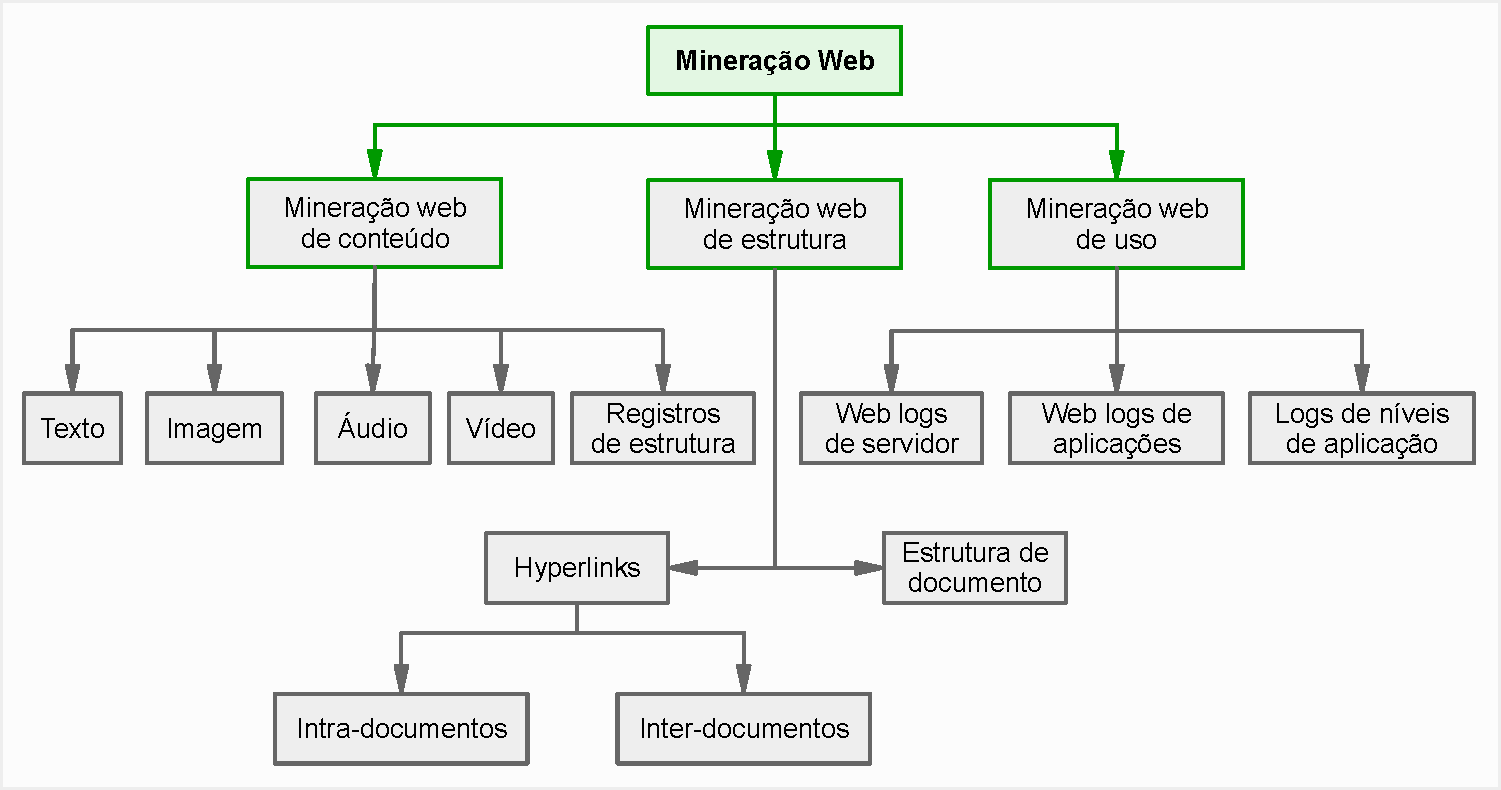
\includegraphics[scale=0.6]{img/taxonomia}\\\vspace{-0.1em}\fonte{\cite{patel_2011}}
		\end{figure}
		
		
		Pretende-se utilizar as ferramentas fornecidas pela mineração Web
		de conteúdo e mineração Web de uso. Esta escolha deve-se a dois fatores;
		o primeiro é a utilização de Web logs (obtidos de \url{https://dumps.wikimedia.org/other/pagecounts-raw/})
		para melhorar a experiência do usuário na busca por conteúdo na Wikipédia,
		e o segundo fator, é a utilização de métodos de Web scraping que se
		aplicam em páginas de artigos acadêmicos semelhantes à Wikipédia.
		Web scraping é um conjunto de técnicas computacionais que são utilizadas
		para obter informação diretamente de páginas Web utilizando requisições
		HTTP.
		
		Finalmente, chegando neste ponto, a estruturação teórica pára e em
		consequência uma ficha da rede de Petri fica no estado da mineração
		Web de conteúdo e a outra, na mineração Web de uso. Com a parte teórica
		consolidada, na subsecção seguinte, explica-se sobre o software que
		é utilizado na parte prática da aplicação Web proposta no trabalho. 
		
		
		\subsection{Bibliotecas de Python utilizadas}
		
		\label{sec:python_biblio}
		
		Esta secção não tem como intenção explicar sobre as funcionalidades
		e recursos básicos linguagem Python, senão, a intenção é expor sobre
		as bibliotecas necessárias que se utilizam para conseguir o objetivo
		estabelecido na presente monografia.
		
		Scrapy, Requests e Beautiful Soup são três bibliotecas open source
		utilizadas para realizar a descoberta de informação na Web de artigos
		relacionados com a Wikipédia, um resumo sobre a funcionalidade dessas
		bibliotecas são mostradas seguidamente:
		
		\begin{description}[style=multiline,leftmargin=3.3cm]
			
			\item [{Scrapy}] É um framework escrito em Python para fazer rastreadores
			Web (Web crawling) mediante a criação de “spiders” que são robôs que
			coletam informação de uma determinada página Web.
			
			\item [{Requests}] É uma biblioteca HTTP para Python, que faz requisições
			Web e extração de conteúdo de uma página Web, essa extração é direta,
			ou seja não existem filtros de tags. Para a filtragem utiliza-se a
			biblioteca Beautifull Soup.
			
			\item [{Beautiful Soup}] É uma biblioteca de Python que serve, principalmente,
			para extrair dados de documentos HTML e XML. A extração de dados é
			realizada utilizando expressões regulares.
			
		\end{description}
		
		Para a etapa de análise dos dados coletados de Web logs da Wikipédia
		utilizam-se as seguintes bibliotecas open source: Scipy, Numpy, Matplotlib
		e Jupyter. Uma breve explicação sobre o funcionamento daquelas bibliotecas
		é exposta em seguida:
		
		\begin{description}[style=multiline,leftmargin=2.5cm]
			
			\item [{SciPy}] Coleção de ferramentas programadas em Python focadas
			para cientistas da computação e analistas.
			
			\item [{NumPy}] Ferramentas oferecidas para resolver problemas computacionais
			relacionados com álgebra linear e transformadas de Fourier.
			
			\item [{Matplotlib}] É uma biblioteca de Python para fazer gráficos
			em duas dimensões. Utiliza-se geramente com a feramenta Jupyter para
			aplicações Web relacionadas com a produção de gráficos semelhantes
			à Mathematica\textregistered
			
			\item [{Jupyter}] É uma aplicação Web que permite criar e compartilhar
			documentos que tenham código, equações, visualizações e textos explicativos.
			Inclui ferramentas como limpeza de dados, simulações numéricas, modelagem
			estatística e aprendizado de máquina.
			
		\end{description}
		
		O resultado final é uma interface Web produzida inteiramente na linguagem
		Python (versão 3.5) utilizando o framework Django onde são implementadas
		as rotinas para a obtenção de dados, o preprocessamento, agrupamento,
		análise, obtenção de conhecimento e reconhecimento de padrões de artigos
		relacionados com a Wikipédia e os Web logs dos servidores desta.
		
		
		
		
		\section{Materiais e métodos}
		
		\label{sec:materiais_metodos}
		
		Como foi exposto na \cref{sec:python_biblio}, utiliza-se a linguagem
		Python (versão 3.5) com as suas respectivas bibliotecas para realizar
		todas as tarefas descritas na secção 4.5. O programa final produzido
		será executado num servidor Web fornecido por Digital Ocean (serviço
		de computação na nuvem) com a interação do usuário final.
		
		Mostram-se, como explicado na \cref{sec:mineracao_dados}, as etapas
		do desenvolvimento do trabalho utilizando a metodologia CRISP-DM:
		
		
		
		\begin{description}[style=multiline,leftmargin=3.5cm]
			
			\item [{Compreensão do negócio }] Deseja-se aprimorar as buscas
			de artigos acadêmicos dos usuários baseando-se na mineração de Web
			logs da wikipédia e na mineração de páginas Web relacionadas. Utiliza-se
			a técnica de mineração de dados porque as informações das páginas
			Web maiormente tem informações irrelevantes. 
			
			\item [{Compreensão dos dados}] Os dados vem de duas fontes: Web
			logs da Wikipédia, que são dados homogêneos e da mineração Web de
			conteúdo de artigos acadêmicos, que são dados heterogêneos.
			
			\item [{Preparação dos dados}]A aplicam-se técnicas de filtragem
			nos bancos de dados de Web logs da Wikipédia e os que foram obtidos
			a través da mineração Web, onde o “ruido” não desejado é eliminado.
			Também aplicam-se técnicas de agrupamento de dados, tudo isso é para
			poder otimizar o treinamento da rede neural que é modelada no passo
			seguinte.
			
			\item [{Modelagem}]Nesta etapa, projeta-se uma rede neural adequada
			ao problema a ser resolvido. A rede neural é do tipo RBF (Radial Basis
			Function) e é implementada tendo como referência o artigo \cite{petprasit_2015}. 
			
			\item [{Avaliação}]Esta etapa realiza-se juntamente com a da Modelagem,
			é dizer, enquanto se projeta uma rede neural ela é testada para verificar
			o cumprimento dos requisitos de solução do problema.
			
			\item [{Desenvolvimento}]Finalmente, o desenvolvimento da aplicação
			Web tendo em conta o anterior mencionado. Destacando que o desenvolvimento
			realiza-se utilizando a técnica TDD\nomenclature[TDD]{TDD}{Test-Driven Development}. 
			
		\end{description}
		
		Depois de haver estabelecido a metodologia, estabelecem-se as atividades
		da aplicação Web proposta no trabalho. Primeiramente, o usuário faz
		uma requisição HTTP no momento de fazer uma busca usando o sistema
		Web proposto, essa ação ativará a busca em vários sites (relacionados
		com artigos acadêmicos) utilizando os métodos de Web scraping, para
		extrair dados da Web é utilizado o algoritmo Subject Detection and
		Node Density proposto em \cite{petprasit_2015}. Em seguida, os dados
		obtidos são armazenados em um banco de dados não relacional (neste
		caso MongoDB) e analisam-se, utilizando uma técnica de rede neural
		supervisionada, juntamente com outros dados que são os Web logs da
		Wikipédia \cref{fig:arquivo_wiki} que já estão armazenados no mesmo
		banco de dados. Finalmente, a resposta preparada é mostrada para o
		usuário, dita resposta contém links de páginas Web de artigos acadêmicos
		que estão relacionados com as palavras chaves da busca. Essas atividades
		são mostradas na rede de Petri da \cref{fig:petri_funcionamento}.
		
		\captionsetup{width=0.7\textwidth}
		\begin{figure}[H]
			\noindent \centering{}\caption{Formato geral de um arquivo de Web log obtido da Wikipédia. \label{fig:arquivo_wiki}}
			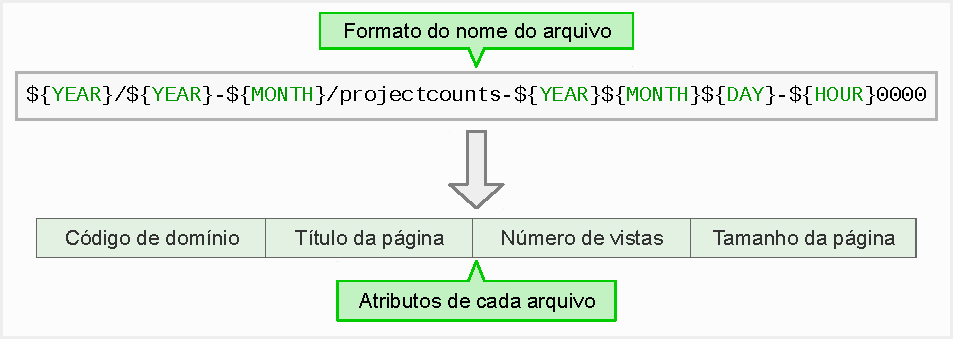
\includegraphics[scale=0.65]{img/modelo_arquivo_wikipedia}\\\vspace{-0.1em}\fonteProp
		\end{figure}
		
		
		\captionsetup{width=0.7\textwidth}
		\begin{figure}[h]
			\noindent \centering{}\caption{Rede de Petri onde mostram-se as atividades da aplicação Web proposta
				no trabalho. \label{fig:petri_funcionamento}}
			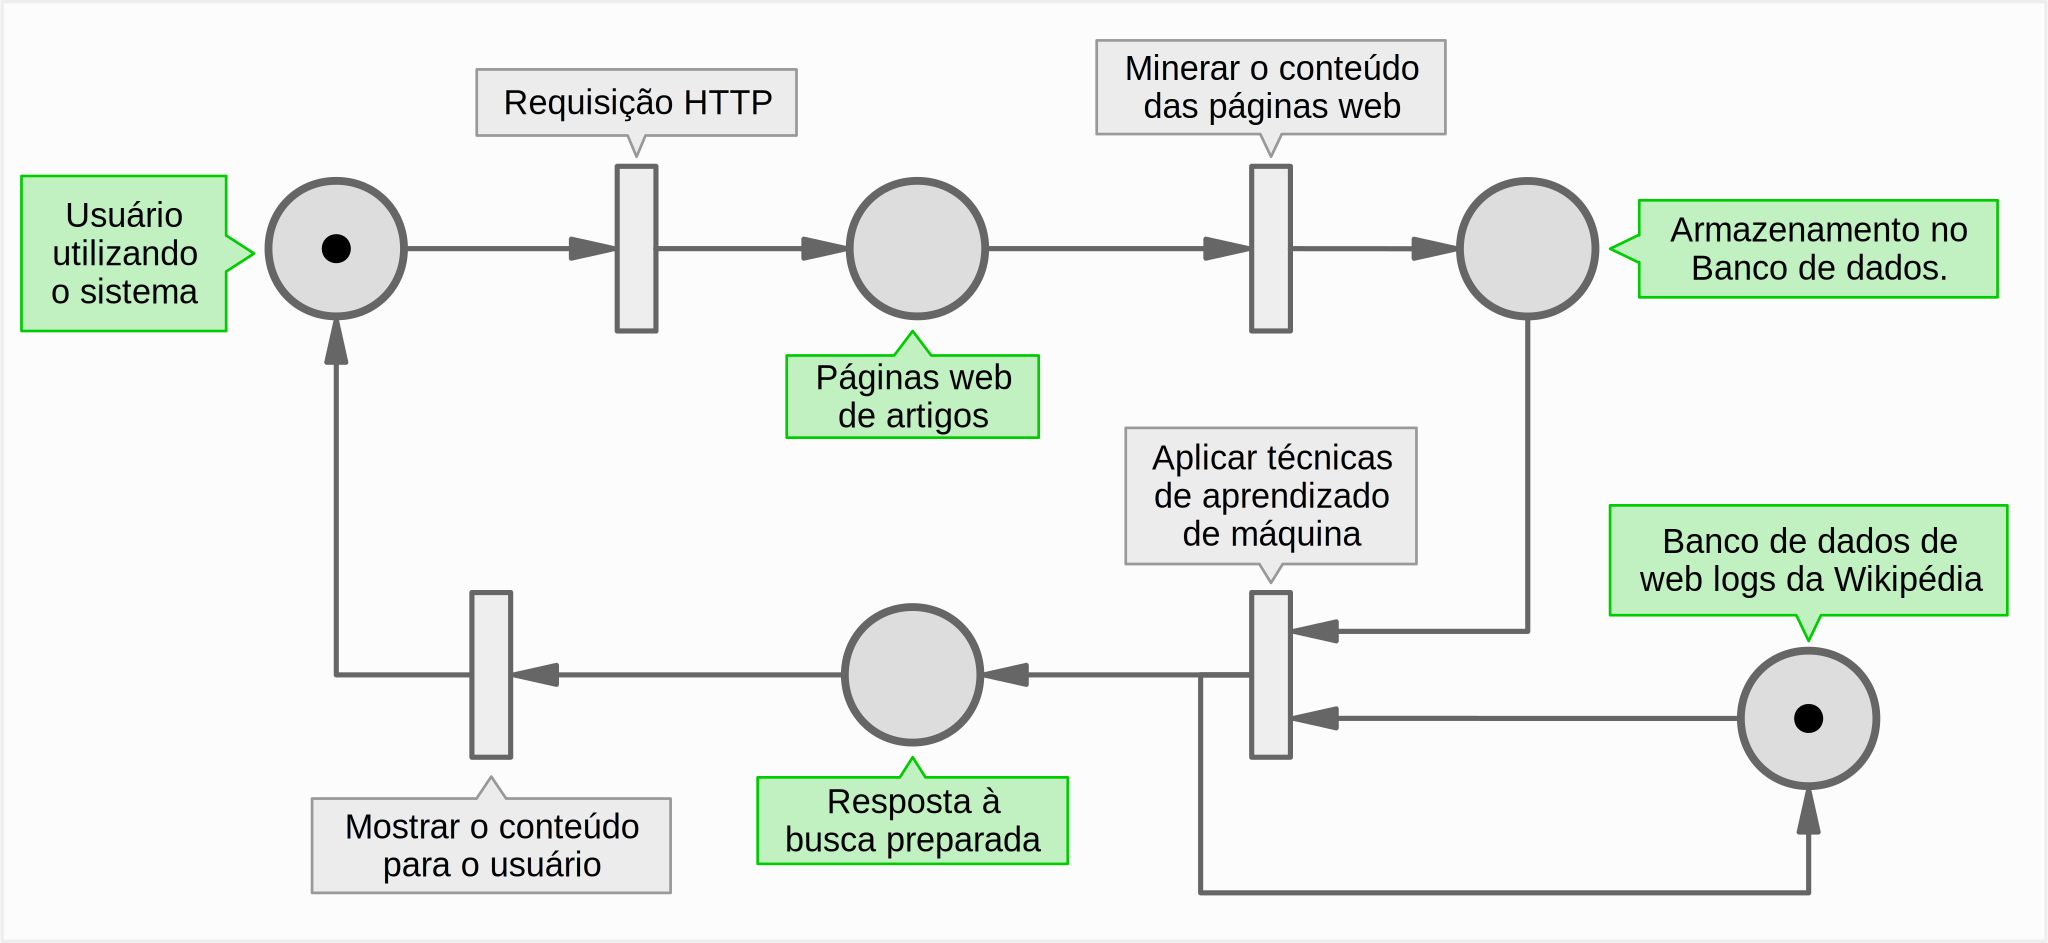
\includegraphics[scale=0.55]{img/rede_petri_funcionamento}\\\vspace{-0.1em}\fonteProp
		\end{figure}
		
		
		Na \cref{tab:cronograma} mostra-se uma previsão de tempo para poder
		realizar todas as tarefas. Lembrando que o processo CRISP-DM, veja-se
		\cref{fig:CRISP-DM}, é cíclico e iterativo.
		
		\captionsetup{width=0.7\textwidth}
		\begin{table}[H]
			\noindent \centering{}\caption{Cronograma que se segue no trabalho de conclusão do curso. \label{tab:cronograma}}
			\begin{tabular}{>{\centering}m{5.3cm}>{\centering}m{5.5cm}}
				\toprule 
				\textbf{Atividade} & \textbf{Data}\tabularnewline
				\midrule
				\midrule 
				Compreensão do negócio  & 01/06/2016 $\longrightarrow$ 14/07/2016\tabularnewline
				\midrule
				Compreensão dos dados  & 15/07/2016 $\longrightarrow$ 02/08/2016\tabularnewline
				\midrule
				Preparação dos dados  & 03/08/2016 $\longrightarrow$ 14/08/2016\tabularnewline
				\midrule
				Modelado, Avaliação, desenvolvimento e TDD  & 15/08/2016 $\longrightarrow$ 15/09/2016\tabularnewline
				\bottomrule
			\end{tabular}\\\vspace{0.1em}\fonteProp
		\end{table}
		
		
		\clearpage{}
		
		%\cleardoublepage
		\phantomsection
		
		\bibliographystyle{abntex2-alf}
		\addcontentsline{toc}{section}{\refname}\bibliography{biblio_bas_seminario_monografia}
		
	\end{document}
